\section{Design requirements}

Houben et al.'s proposed device shown on figure \ref{fig:old-hypr} was taken as a reference, with regards to weight, thickness and size. Although the new design retains the same purpose, the feature of having a dock for a tablet was removed, to further reduce the size. The hybrid patient record was then reimagined to be just a thin support for a folder, with electronics on the back. 

Working from Houben et al.'s proposed device, a new set of requirements have been established, in order to improve on the design. The following list of requirements were decided:

\begin{itemize} \itemsep0em
  \item The individual entries are indicated with a black dot, a so-called bullet.
  \item The text in the entries may be of any length.
\end{itemize}

Numbered list of product requirements with most important first, least important last.

Physical requirements
- lightweight
- small / thin
- maintainability 
	- quickly upload new sofware
	- as close to pick and place as possible
	- easy to change components

Electronic requirements
- rechargeable battery via standard USB cable
- battery status
- long autonomy 
- easy to see LED colours from distance
- easy to hear the audio signal
- ability to connect to wifi
- ability to red RFID tags

\begin{figure}[h]
\begin{center}
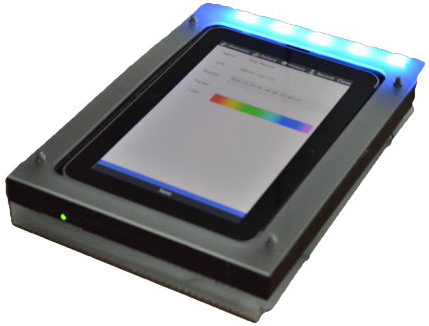
\includegraphics[scale=.5]{figures/old-hypr.jpg}
\caption{\small {\it {This is a description}}} \label{fig:old-hypr}
\end{center}
\end{figure}